\chapter{Streamlining the development of parallel algorithms using Noarr}
\label{chap:noarr}

Commonly, the core computation of scientific algorithms is centered around a master data structure. The examples include a matrix composed of cell features in an agent-based simulator~\cite{ghaffarizadeh2018physicell}, a grid of substrates in a diffusion solver~\cite{ghaffarizadeh2016biofvm}, a transition rates graph for Markov processes~\cite{koltai2020exact}, etc. In the vast majority of these algorithms, the location of the most performance-critical parts lies in a nested loop over these data structures.

Arguably, given a nested loop to optimize, the expert in the performance optimization domain can pinpoint the biggest bottlenecks w.r.t. memory and propose close to optimal modifications with great probability. The problematic activity here, which takes the most programmers time, is putting these modifications into code. For example, let us have a nested loop of depth 3 with control variables \texttt{i, j, k} and bounds \texttt{I, J, K}. A simple tiling modification of the loop adds complexity in loop depth, variable count, and index computation:
\begin{minted}[fontsize=\footnotesize,breaklines,frame=leftline,linenos]{c++}
  for (i1 = 0; i1 < I / tile_I; i1++)
    for (j1 = 0; j1 < J / tile_J; j1++)
      for (k1 = 0; k1 < K / tile_K; k1++)
        for (i2 = 0; i2 < tile_I; i2++)
          for (j2 = 0; j2 < tile_J; i2++)
            for (k2 = 0; k2 < tile_K; k2++)
              // i=i1*tile_I+i2; j=j1*tile_J+j2; k=k1*tile_K+k2;
\end{minted}
Omitting corner cases, the code is already verbose and rather error-prone (a careful eye may spot a mistake, a usual copy-paste bug on Line~$5$).
Naturally, the complexity of the code grows with the complexity of the optimization.

Thankfully, many tools have been developed to alleviate this issue. Some provide automatic optimizations built within a compiler~\cite{trifunovic2010graphite,grosser2012polly}, some extend a compiler with pragma-like annotations to guide the optimization process~\cite{donadio2005language,yi2007poet,chen2008chill,namjoshi2016loopy} and others include ad-hoc solutions for a specific family of algorithms~\cite{9485033,AFANASYEV2021100707}. However, very little attention has been paid to aiding HPC programmers in writing the optimized code from scratch by providing them with a clean and maintainable way to express complex loop traversal and memory layout fit for their specific problem.

To alleviate and streamline the mundane programming tasks repeatedly encountered during our work on optimizing scientific algorithms, we focused our work on developing a C++ library \emph{Noarr}. The main benefit of the library is that it allows to expressively and extensively define memory layouts of regular $n$-dimensional arrays and provides loop transformation primitives for their optimal traversal. It empowers HPC experts to swiftly develop their optimizations as a clean, maintainable code open to autotuning and parallelism while staying within the borders of the C++ standard.


\section{Memory Layouts}
\label{sec:layouts}

Generally, the way how data is laid in memory, a \emph{memory layout}, can be portrayed as a projection of its index space to a linear memory space.

As alluded to in the motivation, common layouts used to optimize memory accesses require a complex code. A tiled matrix layout (Figure~\ref{fig:layout-tile}), the layout paramount for some algorithms to optimally use cache hierarchies, already requires a verbose indexing function. Helping ourselves with adding two intra-tile dimensions, the indexing function would look as follows:
$$L_{\text{tiled}}(i,j,k,l) = (((i \cdot d_2 + j) \cdot d_3) + k) \cdot d_4 + l$$
Arguably, adding another tile dimension, swapping intra-tile layout to column-major form, or implementing layouts as space-filling curves (Figures~\ref{fig:layout-zcurve} and~\ref{fig:layout-hcurve}) becomes less and less trivial. Moreover, considering the indexing functions are written ad-hoc, the layouts are tough subjects to change since a layout change requires a thoughtful and error-prone rewrite of all index function occurrences. On top of that, a complex indexing function is far from self-describing, making it hard, even close to impossible, to guess the layout intentions.

\begin{figure}[h]
  \centering
  \begin{subfigure}{.15\textwidth}
      \centering
      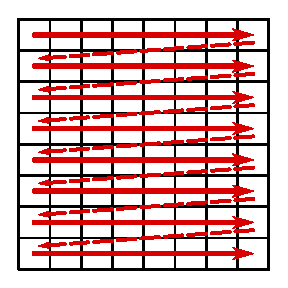
\includegraphics[width=.9\linewidth]{img/matrix-row-major}
      \caption{row-major}
      \label{fig:layout-row}
  \end{subfigure}
  \begin{subfigure}{.15\textwidth}
      \centering
      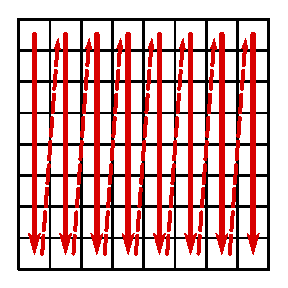
\includegraphics[width=.9\linewidth]{img/matrix-col-major}
      \caption{col-major}
      \label{fig:layout-col}
  \end{subfigure}
  \begin{subfigure}{.15\textwidth}
      \centering
      \includegraphics[width=.9\linewidth]{img/matrix-tiled}
      \caption{tiled}
      \label{fig:layout-tile}
  \end{subfigure}
  \begin{subfigure}{.15\textwidth}
      \centering
      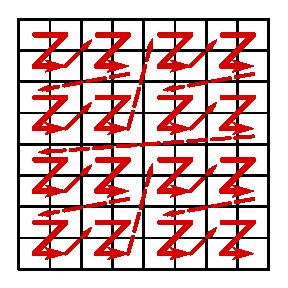
\includegraphics[width=.9\linewidth]{img/matrix-zcurve}
      \caption{z-curve}
      \label{fig:layout-zcurve}
  \end{subfigure}
  \begin{subfigure}{.15\textwidth}
      \centering
      \includegraphics[width=.9\linewidth]{img/matrix-hcurve}
      \caption{Hilbert curve}
      \label{fig:layout-hcurve}
  \end{subfigure}
  \caption{Instances of various matrix layouts.}
  \label{fig:matrix-layout}
  \end{figure}

\subsubsection{Background}

The importance of these issues has been recognized by the HPC community, especially by the authors of HPC programming frameworks. Perhaps the oldest example is Kokkos~\cite{CARTEREDWARDS20143202}, a platform-agnostic programming model that defined a memory layout as a \emph{first-class object}. The layout is defined as a vector of dynamic dimension lengths; the dimensions can be laid out in memory from left to right (Fortran-style), from right to left (C-style) or generally by a custom vector of strides. Such a simple approach covers a wide range of HPC use cases and has been adopted by other frameworks, such as GridTools~\cite{AFANASYEV2021100707}.

Recently, much bigger communities have started to invest time in designing an extensible way of defining layouts. C++ has standardized \emph{mdspan} in C++23. It takes a finer approach, allowing to define layout dimensions using a more complex extent structure. Such a structure enables defining some dimension lengths as static (known at compile time). With such information during compile-time, a compiler can employ optimizations such as constant folding, loop unrolling, or automatized vectorization.

Nvidia has recently introduced \emph{CuTe}, a collection of C++ CUDA template abstractions for defining and operating on hierarchically multidimensional layouts of threads and data~\cite{cute-online}. It follows similar principles as with the C++ standard: it defines \emph{shape}, \emph{stride}, and \emph{tensor} as alternatives to Extents, LayoutPolicy, and mdspan.

\subsection{Noarr Layouts}

Our contribution \emph{Noarr} aims to enhance the expressiveness, extendibility, and maintainability of the code. The main points which distinguish Noarr from other libraries are:

\begin{itemize}
  \item \emph{Named dimensions} --- the dimensions are not defined just by an order of shape or stride vectors, but they are named. This allows to query a dimension regardless of its global index.
  \item \emph{Proto-structures} --- a set of building blocks is provided to allow to easily define complex layouts by their various composition.
\end{itemize}

Let us give an example of a row-major matrix memory layout using Noarr. Considering \mintinline{c++}{'i'} as a row dimension and \mintinline{c++}{'j'} as a column dimension, the layout can be defined as follows:

\begin{minted}[fontsize=\footnotesize,breaklines,frame=leftline,linenos]{c++}
  // Some storage
  int* ptr = new int[80];
  // A row-major matrix layout
  auto row_l = scalar<int>() ^ vector<'j', 'i'>(lit<3>, 4);
  // A bag object with a pointer and a layout
  bag b = make_bag(row_l, ptr);
  int elem = b.at<'i', 'j'>(0, 0);
\end{minted}

Although Noarr predates mdspan and CuTe, it shares many similarities: the separation of layout and underlying memory (using \texttt{bag} on Line~$6$) and the ability to define static and dynamic-sized dimensions (using \texttt{lit} on Line~$4$). Perhaps the biggest difference is the absence of a stride vector. In Noarr, the strides are computed automatically according to the order of the named dimensions:

The order in which the dimensions are defined signals the way how they are laid in memory, which is in the left-to-right fashion. The meaning of the dimension names is important here, as it determines the \emph{logical order}. The order in the definition then defines the \emph{physical order}. For example, let us have a cube layout, denoting its height, width and depth as \mintinline{c++}{'i'}, \mintinline{c++}{'j'} and \mintinline{c++}{'k'} respectively. A C-style cube layout could be defined using \mintinline{c++}{vector<'k', 'j', 'i'>()} proto-structure. A custom layout (neither Fortran- nor C-style) can be simply written as \mintinline{c++}{vector<'j', 'k', 'i'>()}. Using this logical--physical distinction, all of the vastly used stride vectors can be simulated by permuting the dimensions order.

The other aspect of Noarr is the way how the layout is defined --- as a composition of building blocks, the protostructures. We already mentioned \texttt{row\_l}, which is a composition of \mintinline{c++}{scalar<int>} and \mintinline{c++}{vector<'j', 'i'>}, which, when composed, represents a vector (\mintinline{c++}{'i'}) of vectors (\mintinline{c++}{'j'}) of integer scalars (\mintinline{c++}{int}) --- an integer matrix. The left-to-right reading of the layout definition allows for easy extension of the existing layout.

The protostructures allow for expressing complex layouts in a readable and verifiable way. Furthermore, their extensibility in composition and separation from the underlying memory also allows for plug-in layouts, which can be easily \emph{reused} in different parts of the code:

Let us have a complex layout of a multi-layered 3D grid gradient, which occurs on various code places and provides layouts for multiple memory pointers. In that case, a layout can be declared once with sufficient scope and reused in places where needed:

\begin{minted}[fontsize=\footnotesize,breaklines,frame=leftline,linenos]{c++}
  // A globally accessible layout
  auto gradient_layout = scalar<float>()
    ^ vector<'s', 'x', 'y', 'z', 'g'>(
      substrates, grid_dims[0], grid_dims[1], grid_dims[2], lit<3>
    );

  void func1_cpu(float* grad_ptr) {
    bag b = make_bag(gradient_layout, grad_ptr);
    // use the layout on CPU memory
  }

  void func2_gpu(float* global_mem_ptr) {
    bag glb_b = make_bag(gradient_layout, global_mem_ptr);
    bag shm_b = make_bag(gradient_layout, shared_mem_ptr);
    // use the layout on GPU global and shared memory
  }
\end{minted}

The other benefit of having a layout as a reusable first-class object is the ability to have a localized change when deciding to modify the layout code during the implementation. Extending our previous example, if we decide to reorder the gradient dimension \mintinline{c++}{'g'} to be the innermost one, we only change the definition of the object on Line~$2$ --- all the data structures using the layout will be transparently updated without any further code changes.


\section{Traversing Layouts}
\label{sec:traversals}

Having specified how a data structure is laid in memory, the other possible point of optimization lies in the order how the data structure is iterated, its \emph{traversal}. In general, a traversal is usually written as a sequence of nested loops, which in turn generates a sequence of data structure accesses. Therefore, as with a layout, modifying a traversal can improve data locality, both in time and space. Although modifying traversal can be constrained by data dependencies, loop transformation is still a well-researched topic and complements the memory layout optimization~\cite{clauss2000automatic}.

Writing complex traversals complements the issues discussed above when detailing the layouts. So, such tool can share the same benefits: expressivity, maintainability, and reusability. Moreover, since traversing over some master data structures is the common place where parallelism is introduced in the code, the abstraction of loop transformation can further extend to parallel processing.

\subsubsection{Background}

Quantitatively, \emph{loop transformation} is perhaps a more researched topic than layout transformation. Neither library mentioned above provides ways to transform a traversal, but many other tools do. Contemporary compilers employ sophisticated loop optimizers based on the polyhedral model, such as Graphite in GCC~\cite{trifunovic2010graphite} or Polly in LLVM~\cite{grosser2012polly}. However, these optimizers are limited by the lack of information specified by the user in the code.

For more user-guided approaches, there are annotation-based tools, such as Poet~\cite{yi2007poet}, Chill~\cite{chen2008chill} or Loopy~\cite{namjoshi2016loopy}. These tools allow to specify the traversal transformations by adding special comments or pragmas to the code. The transformations are then applied by a precompiler, which generates the optimized code.
These tools are straightforward to use, and their ability to combine them to form complex loop transformations makes them very expressive. A minor downside is that they are typically closed to extensions, and for most of them, a precompiler with an extra preprocessing step or a custom compiler extension is needed.

On the other hand, the target problems for annotation-based loop transformation tools are somehow limited. Naturally, the best use of them is made when there is already a baseline implementation, and the optimization is achieved just by adding a few lines on the top of the loop with the hottest performance spots. However, when developing an optimized solution from scratch and when the scale of the program passes a certain complexity threshold, optimizing just by annotations may become cumbersome~\cite{kegel2009using,ajkunic2012comparison,refsnes2011comparison}.

\subsection{Noarr Traversers}

The similarities in memory layout and its traversal led us to the development of our following contribution, \emph{Noarr Traversers}. The tool is based on the idea that every single loop, in some sequence of nested loops, can be interpreted as one (named) dimension in an index space domain. Assuming perfectly nested loops, such traversal can be interpreted as a Noarr layout and be subjected to the same transformations as a memory layout. To sum up, the key points of Noarr Traversers are as follows:
\begin{itemize}
  \item \emph{Named dimensions} --- a traverser comprises named dimensions, each representing a loop in a sequence of nested loops.
  \item \emph{Proto-structures} --- exactly as with layouts, a traverser is subject to an extension using the same set of proto-structures.
  \item \emph{Index space extraction} --- the traverser extracts dimensions from the passed-in layouts and yields an index space corresponding to the cartesian product of the extracted dimensions.
\end{itemize}

Let us highlight the main idea of Noarr Traverser on an example of matrix multiplication, where a plain C++ implementation would look like this:

\begin{minted}[fontsize=\footnotesize,breaklines,frame=leftline,linenos]{c++}
  for (int i = 0; i < m; i++)
    for (int j = 0; j < n; j++)
      for (int k = 0; k < p; k++)
        C[i][j] += A[i][k] * B[k][j];
\end{minted}
The nested loops follow the order of $3$ present dimensions: $i$, $j$, and $k$ denoting rows of $C$ and $A$, columns of $C$ and $B$, and rows of $A$ and columns of $B$, respectively. Smartly selecting the named dimensions of the layouts, the traversal can be rewritten using Noarr as follows:

\begin{minted}[fontsize=\footnotesize,breaklines,frame=leftline,linenos]{c++}
  auto A = make_bag(ptr_a, scalar<int> ^ vector<'k', 'i'>(K, I));
  auto B = make_bag(ptr_b, scalar<int> ^ vector<'j', 'k'>(J, K));
  auto C = make_bag(ptr_c, scalar<int> ^ vector<'j', 'i'>(J, I));

  traverser(A, B, C) | [=](auto state) {
    C[state] += A[state] * B[state];
  };
\end{minted}
The traverser accepts the layouts (or bags) it shall iterate over. It extracts $3$ unique dimensions \mintinline{c++}{'i'}, \mintinline{c++}{'j'} and \mintinline{c++}{'k'} and iterates over the index space composed of these dimensions as if they were written as a sequence of nested loops (which is equivalent to the cartesian product of these dimensions). The lambda function on Line~$6$ is then executed for each point in the index space, passing the tuple of indices as the \texttt{state} argument to the lambda.

Thanks to the dimension naming, traversers and layout objects are also \emph{isomorphic}. Consequently, changing the traversal order is done the same way as modifying the layout --- by applying the proto-structures to the traverser. E.g., to reorder the loops to a more cache-friendly \mintinline{c++}{'i'}, \mintinline{c++}{'k'}, \mintinline{c++}{'j'} order, the traversal can be rewritten as follows:
\begin{minted}[fontsize=\footnotesize,breaklines,frame=leftline,linenos]{c++}
  traverser(A, B, C) ^ reorder<'i', 'k', 'j'>() | [=](auto state) {
    C[state] += A[state] * B[state];
  };
\end{minted}


\subsubsection{Reusability}

Similarly as with layouts, a specific traversal order can be defined as an object, such as \texttt{tiles} on Line~$2$ in the previous code sample, and provide the same benefits: locality of change and reusal.

But this feature further extends to a perhaps more powerful concept, which we call \emph{layout agnosticism} and \emph{traversal agnosticism}. As a case of the separation of concerns, a memory layout and traversal can be extracted from a function to the level of function arguments. These arguments may then serve as interfaces for the concrete traversal or layout objects:

\begin{minted}[fontsize=\footnotesize,breaklines,frame=leftline,linenos]{c++}
  template <class A_t, class B_t, class C_t, class Order_t>
  void matmul(A_t& A, B_t& B, C_t& C, Order_t my_order)
  {
      traverser(A, B, C) ^ my_order | [=](auto state) {
          C[state] += A[state] * B[state];
      };
  }
\end{minted}
The function \mintinline{c++}{matmul} becomes agnostic to the layout or traversal specified, and, regardless of the passed-in objects, it will run the same operations, just in a different order.

\subsubsection{Parallelism}

Since Noarr is general enough to allow the division of traversals into independent sub-traversals, the user can also guide the parallelism of a program. Proto-structures such as \mintinline{c++}{fix}, \mintinline{c++}{slice} or \mintinline{c++}{step} provide expressive ways to split a work over a data structure into custom sections. The user can then assign each section to a separate thread, which will iterate over the section independently.

The following code sample further strengthens the benefit of named dimensions: The user can directly specify the dimension to parallelize over. This is even more visible when targeting parallel accelerators (such as GPUs) in which a programmer can select multiple dimensions to utilize thread hierarchies (as described in \cref{sec:gpu_arch}):

\begin{minted}[fontsize=\footnotesize,breaklines,frame=leftline,linenos]{c++}
  auto A = make_bag(ptr_a, scalar<int>() ^ vector<'x', 'y'>(32, 1000));
  // spawns a cuda block for each element of the 'y' dimension
  // with as many threads as the size of 'x' dimension
  auto ct = noarr::cuda_threads<'y', 'x'>(traverser(A));
  a_kernel<<<ct.grid_dim(), ct.block_dim()>>>(ct.inner(), A);

  __global__ void a_kernel(auto traverser, auto A) {
    // A is accessed according to the block index
    // and the thread index of the currently executing thread
    auto var = A[traverser.state()];
  }
\end{minted}

\section{Summary}

With the arsenal of proto-structures, Noarr provides options to specify many complex layouts and traversals. The object-oriented design of the library allows writing complex memory optimizations in an extensible, reusable, and even layout-agnostic way, with very little space for errors. Further, the pure C++ implementation enables the usage of Noarr in C++-based frameworks, such as CUDA. We believe that our solution will add a new expressive tool to a high-performance programming toolset, simplifying the research focusing on tuning of prewritten computational kernels and building complex optimized parallel algorithms from scratch.
